%15 min preso!
\documentclass[xcolor=table,aspectratio=169]{beamer}
\usepackage{beamerthemesplit}
\usepackage{wrapfig}
\usetheme{SPbGU}
\usepackage{pdfpages}
\usepackage{amsmath}
\usepackage{cmap}
\usepackage[T2A]{fontenc}
\usepackage[utf8]{inputenc}
\usepackage[english]{babel}
\usepackage{indentfirst}
\usepackage{amsmath}
\usepackage{tikz}
\usepackage{multirow}
\usepackage[noend]{algpseudocode}
\usepackage{algorithm}
\usepackage{algorithmicx}
\usepackage{fancyvrb}
\usepackage{hyperref} 
\usetikzlibrary{calc}
\usetikzlibrary{shapes}
\usetikzlibrary{arrows,automata}
\usetikzlibrary{positioning}
\usetikzlibrary{fit}
\usetikzlibrary{shapes.callouts}
\usetikzlibrary{shapes.misc}
\usepackage{xparse}

\usepackage{etoolbox,refcount}
\usepackage{multicol}

\usepackage{tabularx}
\newcolumntype{Y}{>{\raggedleft\arraybackslash}X}

\renewcommand{\thealgorithm}{}

\newtheorem{mytheorem}{Theorem}
\renewcommand{\thealgorithm}{}

\newcommand{\tikzmark}[1]{\tikz[overlay,remember picture] \node (#1) {};}
\def\Put(#1,#2)#3{\leavevmode\makebox(0,0){\put(#1,#2){#3}}}

\newcommand{\ltz}{$< 1$}

\tikzset{
    state/.style={
           rectangle,
           rounded corners,
           draw=black, very thick,
           minimum height=2em,
           inner sep=2pt,
           text centered,
           },
}

\tikzset{
    invisible/.style={opacity=0,text opacity=0},
    visible on/.style={alt=#1{}{invisible}},
    alt/.code args={<#1>#2#3}{%
      \alt<#1>{\pgfkeysalso{#2}}{\pgfkeysalso{#3}} % \pgfkeysalso doesn't change the path
    },
}

\tikzset{cross/.style={cross out, draw=black, minimum size=2*(#1-\pgflinewidth), inner sep=0pt, outer sep=0pt, ultra thick},
%default radius will be 1pt. 
cross/.default={1pt}}

\NewDocumentCommand{\mycallout}{r<> O{opacity=0.8,text opacity=1} m m m}{%
\tikz[remember picture, overlay]\node[align=center, fill=cyan!20, text width=#5cm,
#2,visible on=<#1>, rounded corners,
draw,rectangle callout,anchor=pointer,callout relative pointer={(290:0.5cm)}]
at (#3) {#4};
}

\NewDocumentCommand{\mycalloutR}{r<> O{opacity=0.8,text opacity=1} m m m}{%
\tikz[remember picture, overlay]\node[align=center, fill=cyan!20, text width=#5cm,
#2,visible on=<#1>, rounded corners,
draw,rectangle callout,anchor=pointer,callout relative pointer={(30:0.8cm)}]
at (#3) {#4};
}


%callout relative pointer={(230:0.5cm)}]

\newcounter{countitems}
\newcounter{nextitemizecount}
\newcommand{\setupcountitems}{%
  \stepcounter{nextitemizecount}%
  \setcounter{countitems}{0}%
  \preto\item{\stepcounter{countitems}}%
}
\makeatletter
\newcommand{\computecountitems}{%
  \edef\@currentlabel{\number\c@countitems}%
  \label{countitems@\number\numexpr\value{nextitemizecount}-1\relax}%
}
\newcommand{\nextitemizecount}{%
  \getrefnumber{countitems@\number\c@nextitemizecount}%
}
\newcommand{\previtemizecount}{%
  \getrefnumber{countitems@\number\numexpr\value{nextitemizecount}-1\relax}%
}
\makeatother    
\newenvironment{AutoMultiColItemize}{%
\ifnumcomp{\nextitemizecount}{>}{3}{\begin{multicols}{2}}{}%
\setupcountitems\begin{itemize}}%
{\end{itemize}%
\unskip\computecountitems\ifnumcomp{\previtemizecount}{>}{3}{\end{multicols}}{}}


\beamertemplatenavigationsymbolsempty

\title[High-Performance Graph Analysis]{Linear Algebra Based High-Performance Graph Analysis}
\institute[SPbSU]{
Saint Petersburg State University
}

% То, что в квадратных скобках, отображается в левом нижнем углу.
\author[Semyon Grigorev]{Semyon Grigorev}

\date{June 7, 2023}

\begin{document}
{
\begin{frame}[fragile]
  \begin{table}
  \centering
  
\includegraphics[height=1.5cm]{pictures/SPbGU_Logo.png}
  %\begin{tabularx}{\linewidth}{XcX}
    %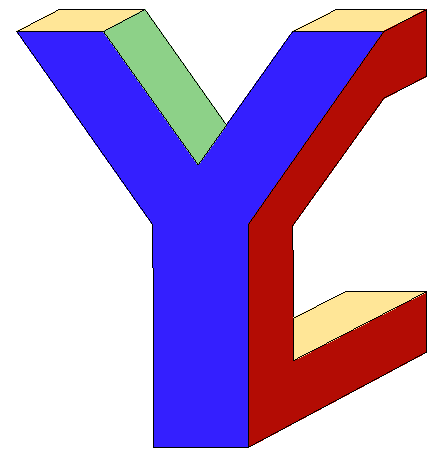
\includegraphics[height=1.5cm]{pictures/YC_logo.pdf} \hfill
    %& \begin{minipage}[t]{0.3\textwidth}\center \vspace{-1cm}  %Huawei-SPbSU Open Day 2021
    %  \end{minipage}
    %& \hfill 
\includegraphics[height=1.5cm]{pictures/SPbGU_Logo.png}
  %\end{tabularx}
  \end{table}
  \titlepage
\end{frame}
}


\begin{frame}[fragile]
  \frametitle{Research areas}
  \begin{itemize}
    \item Linear algebra based algorithms for graph analysis
    \begin{itemize}
      \item GraphBLAS-based algorithms design, implementation and evaluation
      \item Portable multi-GPGPU implementation of GraphBALS-like API
      \item GraphBLAS API analysis
    \end{itemize} 
    \item Path problems with constraints
    \begin{itemize}
      \item Formal Language Constrained Path Querying
      \begin{itemize}
        \item New algorithms development
        \item Complexity analysis
        \item New classes of languages investigation
        \item High performance algorithms implementation and evaluation 
      \end{itemize}
    \end{itemize}
  \end{itemize}
\end{frame}

\begin{frame}[fragile]
  \frametitle{Our Results}
    \begin{itemize}
      \item Tools
      \begin{itemize}
        \item \href{presentation_graph_analysis}{Spla: generalized sparse linear algebra framework with vendor-agnostic GPUs accelerated computations}
        \item \href{https://github.com/SparseLinearAlgebra/spbla}{SPbLA: library of GPGPU-powered sparse boolean linear algebra operations}    
        \item \href{https://github.com/FormalLanguageConstrainedPathQuerying/CFPQ_PyAlgo}{CFPQ\_PyAlgo: set of GraphBLAS-based FLPQ algorithms}
        \item \href{https://github.com/FormalLanguageConstrainedPathQuerying/GLL4Graph}{GLL4Graph: CFPQ for Neo4j}
        \item \href{https://github.com/YaccConstructor/RedisGraph}{CFPQ for RedisGraph}
      \end{itemize}
      \pause
      \item Papers (> 10)
      \begin{itemize}
        \item SPbLA: The Library of GPGPU-Powered Sparse Boolean Linear Algebra Operations (GrAPL@IPDPS)
        \item Evaluation of the context-free path querying algorithm based on matrix multiplication (GRADES-NDA@SIGMOD)
        \item Multiple-Source Context-Free Path Querying in Terms of Linear Algebra (EDBT, Core A)
        \item Context-free path querying by matrix multiplication (GRADES-NDA@SIGMOD)
      \end{itemize} 
    \end{itemize}
\end{frame}


\end{document}
